\subsection{Overall System Architecture}

The embedded system architecture connects the microscope, mechanical adapters, electronics, camera input, touchscreen, and software into one control platform. The Raspberry Pi acts as the central computer. It runs the Python/PySide application, renders the QML interface, receives camera frames, communicates with the motor controller, reads user input devices, stores captures, and exposes the REST API. The motor controller drives the stepper motors for the XY stage and focus axis. Additional devices provide joystick input, focus encoder input, buttons, endstop, and optional current sensing.

The system is intentionally modular. Hardware-specific behavior is isolated in drivers, application behavior is implemented in services, pure calculations are placed in domain modules, bridge classes expose state and commands to QML, and the QML files implement the touch interface. This separation makes the system easier to test and modify. It also supports mock mode, where parts of the system can run without the physical microscope.

\subsection{Hardware Selection and Cost Constraints}

The prototype hardware was selected under low-cost and reproducibility constraints. The selected components include a Raspberry Pi 4, DSI touchscreen, Elgato Cam Link, Sangaboard, 28BYJ-48 stepper motors, analog joystick, ADS1115 analog-to-digital converter, incremental rotary encoder, endstop, and buttons.

The Sangaboard was selected as the dedicated motor-controller board. In this thesis, Sangaboard is an open-source motor controller placed between the Raspberry Pi and the stepper motors: it receives serial commands from the host over UART, drives the motor coils, and reports motor step counts back to the application. It is part of the OpenFlexure ecosystem \cite{collins2020openflexure,openflexureDocs}. RetroScope reuses this motor controller for a different purpose: instead of driving a printed OpenFlexure microscope stage, the Sangaboard drives retrofit adapters attached to the existing XY stage and fine-focus mechanism.

The 28BYJ-48 motors were chosen because they are inexpensive and easy to drive. A direct-drive stepper alternative was considered. It would offer easier manual rotation and different mechanical behavior, but it would require a higher-voltage, higher-current supply, a different motor controller, and protection against generated electrical energy when rotated manually. The chosen hardware therefore reflects the thesis goal: explore how far a low-cost retrofit can be pushed rather than eliminating all limitations through more expensive components.

Table~\ref{tab:components} lists the main electronic and mechanical components and their role in the
platform. The priced bill of materials with suppliers and total prototype cost is given in
Appendix~\ref{app:bom}. Exact prices depend on supplier and date.

\begin{table}[H]
    \centering
    \caption[Main hardware components]{Main hardware components of the RetroScope prototype and their role.}
    \label{tab:components}
    \begin{tabular}{@{}L{4.8cm} c L{6.8cm}@{}}
        \toprule
        \textbf{Component} & \textbf{Qty} & \textbf{Role / interface} \\
        \midrule
        Raspberry Pi 4 Model B (4\,GB) & 1 & Central computer, runs the PySide6/QML application and REST API \\
        DSI capacitive touchscreen & 1 & Primary touch user interface \\
        Elgato Cam Link & 1 & UVC video capture of the microscope camera (USB) \\
        Sangaboard motor controller & 1 & Stepper driving and step counting (UART) \\
        28BYJ-48 geared stepper motor & 3 & X-stage, Y-stage, and focus drives \\
        Analog joystick ($2\times10\,\mathrm{k}\Omega$) & 1 & Manual XY motion \\
        ADS1115 ADC module & 1 & Joystick analog-to-digital conversion (I\textsuperscript{2}C) \\
        Incremental rotary encoder & 1 & Manual focus (Z) input \\
        INA219 current-sense module & 2 & Motor current / stall sensing, not used for final control logic (I\textsuperscript{2}C) \\
        Logic-level shifter (BSS138) & 1 & 5\,V\ to 3.3\,V protection for GPIO inputs \\
        Endstop switch & 1 & Focus-axis (Z) safety limit \\
        Push button & 4 & Assignable user actions \\
        Custom PCB & 1 & Consolidates wiring, components, level shifting, and connectors \\
        3D-printed parts (PETG, ABS-GF) & -- & Adapters, motor mounts, brackets, enclosure, ... \\
        \bottomrule
    \end{tabular}
\end{table}

\subsection{Raspberry Pi, Display, Camera, and Video Capture}

The Raspberry Pi provides the computational and interface core of the platform. It runs the QML touchscreen interface and the Python backend, and it connects to the display, camera capture device, motor controller, and peripheral electronics.

Camera input was one of the more difficult implementation areas. The Cam Link appeared as a standard UVC device on Linux. A 4K signal produced too much USB bandwidth for the Raspberry Pi 4, requiring downscaling to 1080p and the camera formats NV12 and YU12 required color conversion. The camera system was structured into multiple paths: a direct preview path for low-latency QML video output, a CPU frame-analysis path at configurable resolution and frame rate, a native still-capture path for full-resolution snapshots and automated captures, and a native recording path for video.

Live preview is seperated from frame analysis. Live video can remain responsive while the analysis path computes histogram values, focus scores, and objective-change metrics at a lower rate. This separation was important because frame analysis originally affected the performance of the live preview and responsiveness of e.g. the joystick.

\subsection{Motor Controller, Stepper Motors, and Input Devices}

The Sangaboard communicates with the Raspberry Pi over UART and controls the stepper motors. Disabling Bluetooth on the Raspberry Pi was necessary to use the full PL011 UART for Sangaboard communication because the mini UART has a smaller FIFO size.

Manual input is provided through a joystick for XY movement and a rotary encoder for focus movement. The joystick uses two potentiometer axes connected through an ADS1115 ADC over I\textsuperscript{2}C. The rotary encoder is used for Z control. A logic-level shifter was necessary because the encoder operates at 5 V while Raspberry Pi GPIO pins are 3.3 V tolerant. The system also includes buttons for user actions such as autofocus or recording, and an endstop to prevent dangerous focus movement, like crashing the objective into the sample.

\subsection{Custom PCB, Wiring, and Power Distribution}

The custom PCB replaces breadboard wiring and makes the prototype more reproducible. The KiCad project in the repository contains schematic, PCB, symbol, Gerber, drill, and STEP files. The schematic and board files show connectors for the Raspberry Pi, joystick/ADC path, INA219 modules, level shifting, endstop/buttons, and power rails. The board uses 5 V and 3.3 V rails and common ground, with I\textsuperscript{2}C shared by several modules.

The two INA219 current-sense modules are included in the final PCB and wiring, but they are not used by the final prototype for motor stall detection. They were originally added to detect abnormal motor load through supply-current changes. In practice, this was not reliable with the unipolar 28BYJ-48 motors and the Sangaboard drive pattern: depending on the current step phase, one or two coils can be energised, so the measured current is dominated by the coil-energising sequence rather than by a clearly readable load or stall signal. The modules are therefore still shown in the hardware list, bill of materials, schematic, and wiring table because they are physically part of the built PCB, but the software does not depend on them for the final motion-control behaviour.

\begin{figure}[H]
    \centering
    \begin{subfigure}[t]{0.48\linewidth}
        \centering
        \includegraphics[width=\linewidth]{images/pcb_board.png}
        \caption{Assembled board.}
    \end{subfigure}\hfill
    \begin{subfigure}[t]{0.48\linewidth}
        \centering
        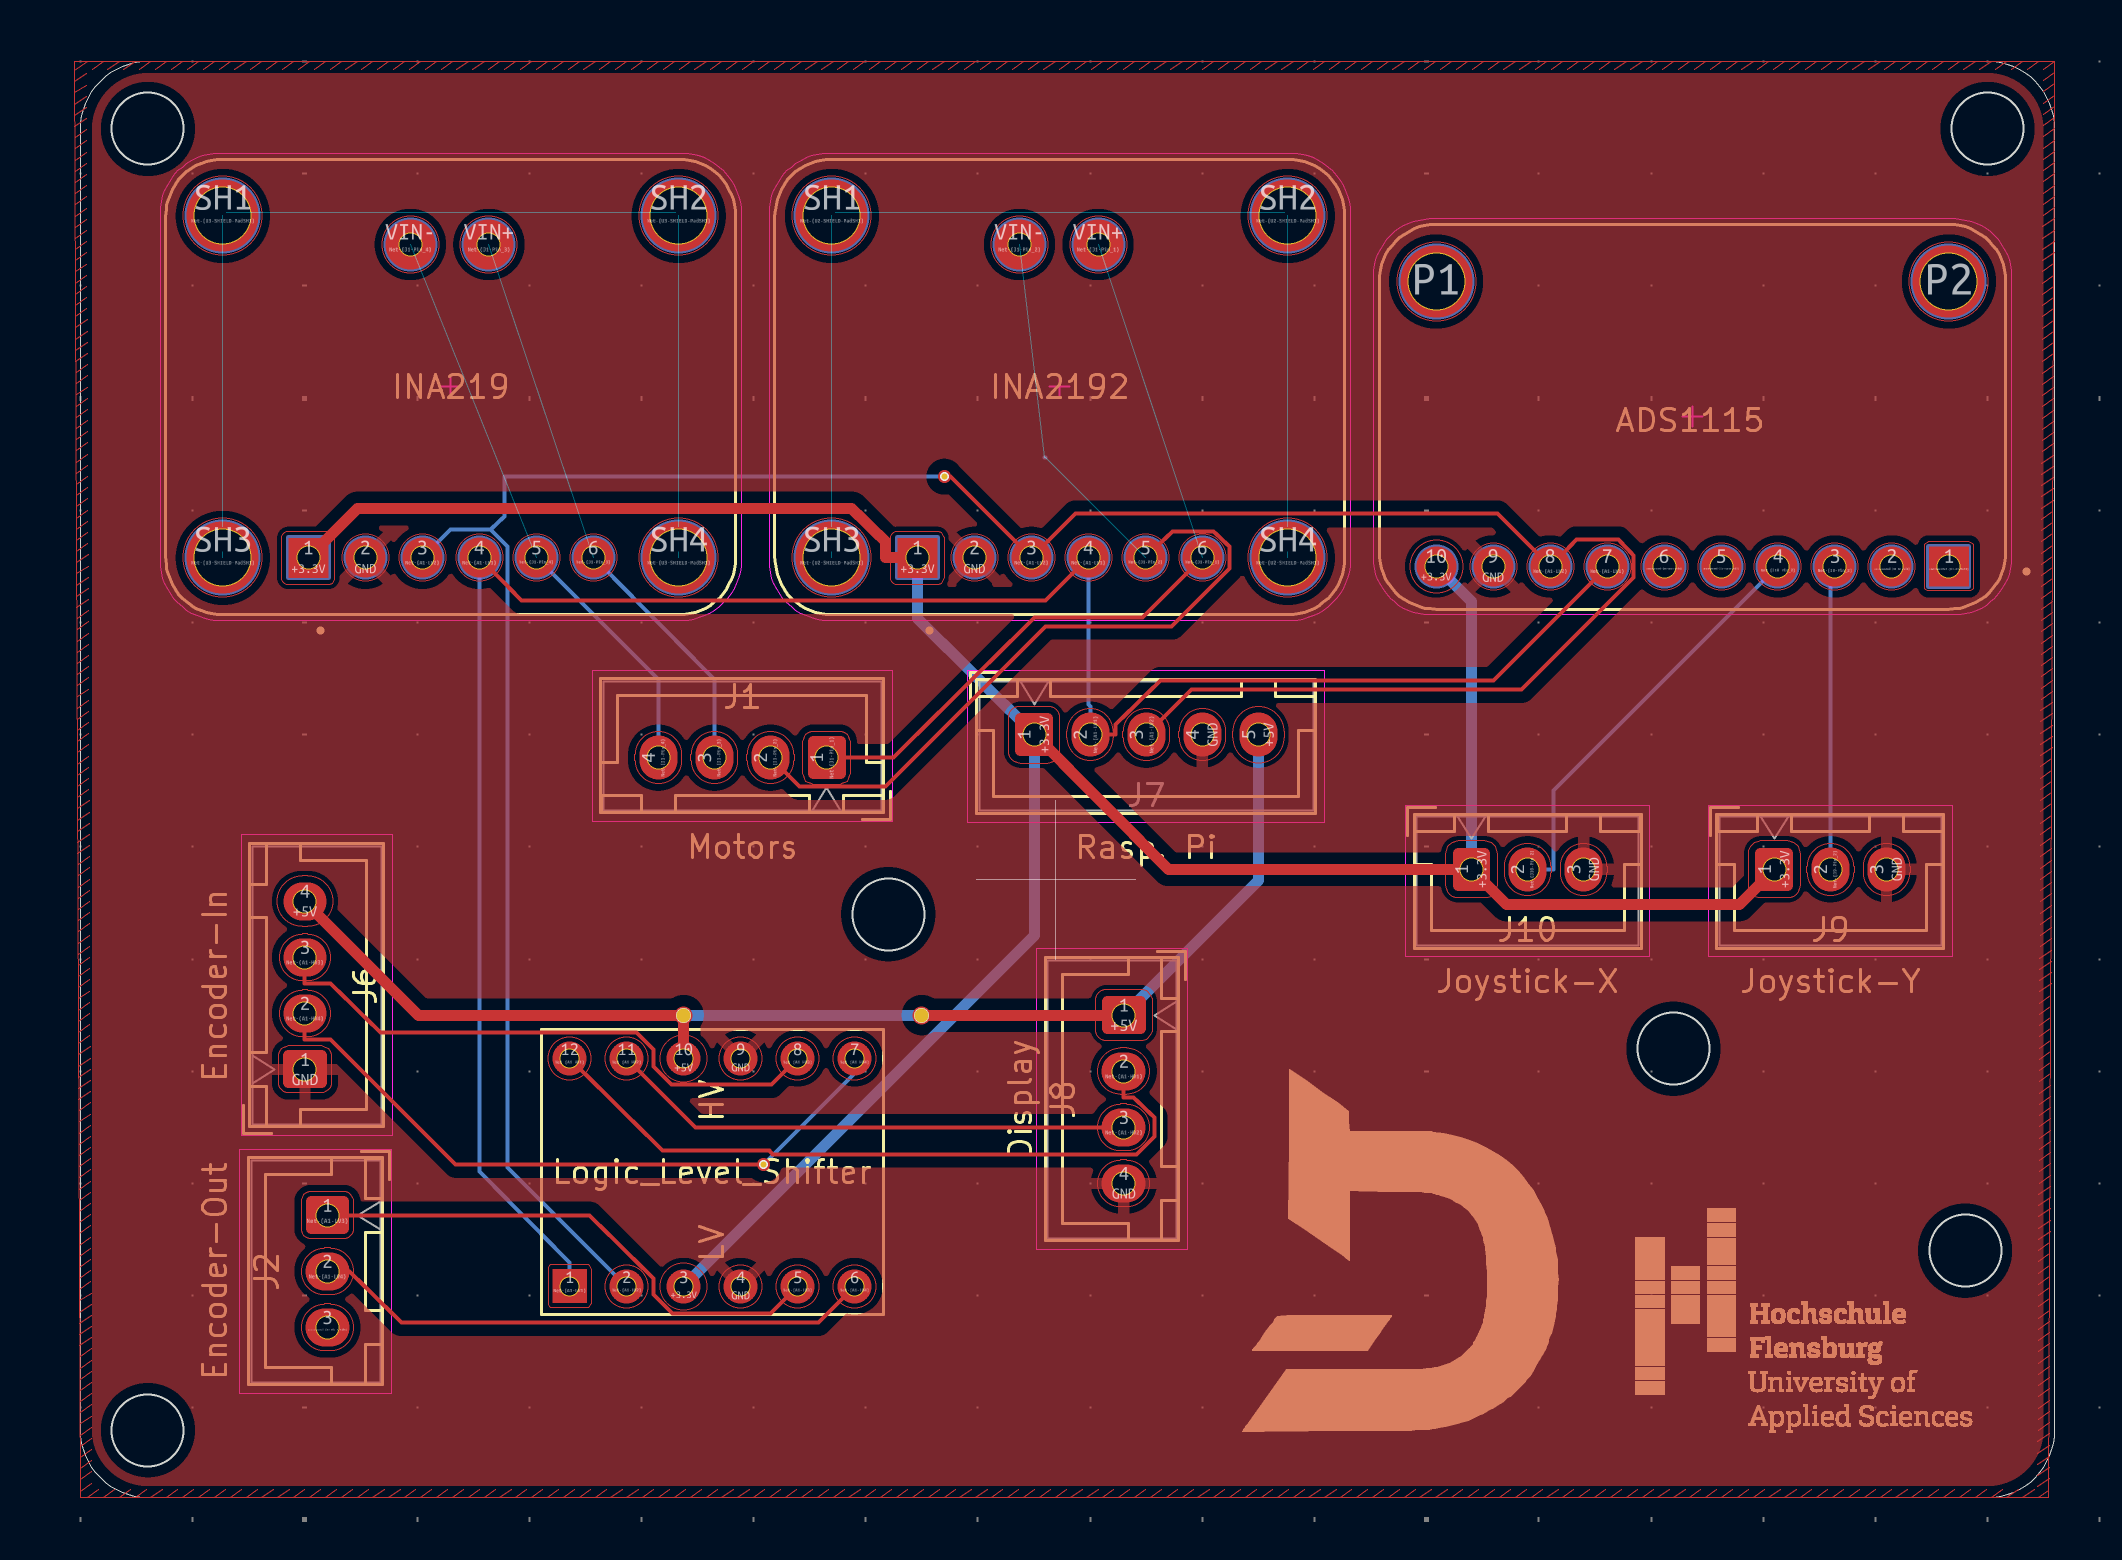
\includegraphics[width=\linewidth]{images/pcb_board2.png}
        \caption{PCB routing with modules, connectors, and power rails.}
    \end{subfigure}
    \caption[Assembled custom PCB]{The assembled RetroScope custom PCB (KiCad design, manufactured via JLCPCB),
    consolidating the joystick ADC, current-sense modules, level shifting, endstop/button
    connectors, and power rails. The board files are listed in Appendix~\ref{app:pcb}.}
    \label{fig:pcb}
\end{figure}

Table~\ref{tab:wiring} summarises the signal routing: the Sangaboard UART,
the level-shifted encoder inputs, the endstop and buttons, the shared I\textsuperscript{2}C bus with
its device addresses, and the power rails. The full pin map and the KiCad/Gerber references are
reproduced in Appendix~\ref{app:wiring} and Appendix~\ref{app:pcb}.

\begin{table}[H]
    \centering
    \caption[GPIO, I2C, UART, and power routing]{GPIO, I\textsuperscript{2}C, UART, and power routing of the prototype (BCM GPIO numbering).}
    \label{tab:wiring}
    \begin{tabular}{@{}L{3.4cm} L{4.3cm} L{6.0cm}@{}}
        \toprule
        \textbf{Subsystem} & \textbf{Pins / address} & \textbf{Notes} \\
        \midrule
        Sangaboard (UART) & GPIO 14 (TXD), 15 (RXD) & Full PL011 UART, Bluetooth disabled to free it \\
        Sangaboard control lines & GPIO 4, 8, 11, 23, 24, 25 & Stepper control / step signalling \\
        Rotary encoder & GPIO 17, 27 & Through 5\,V\ to 3.3\,V level shifter \\
        Endstop & GPIO 16 & Focus-axis (Z) safety limit \\
        Push buttons & GPIO 6, 13, 19, 26 & \\
        I\textsuperscript{2}C bus & GPIO 2 (SDA), 3 (SCL) & Shared by the modules below \\
        \quad ADS1115 & 0x48 & Joystick ADC \\
        \quad INA219 ($\times2$) & 0x40, 0x41 & Current-sense hardware \\
        \quad Touchscreen & 0x38, 0x45 & Touch controller and backlight \\
        Power rails & 5\,V, 3.3\,V, GND & Common ground \\
        \bottomrule
    \end{tabular}
\end{table}

\subsection{Software Layering: Drivers, Services, Domain Logic, and UI Bridges}

The software architecture is separated into layers. Drivers access hardware such as Sangaboard, joystick ADC, encoder, buttons, endstop, and camera sources. Services implement application behavior such as motion control, autofocus, focus stacking, tile scanning, image storage, updates, and REST API lifecycle. Domain modules implement pure calculations such as scan planning, focus metrics, focus blending, and calibration helpers. Bridge classes expose service state and commands to QML using Qt properties, signals, and slots. QML files implement the user interface.

This structure was explicitly motivated by maintainability and expandability.The QML views should not directly depend on low-level services or drivers. A new subsystem can be added by implementing a service or driver, exposing it through a bridge, and connecting it to QML. The design also supports unit testing because domain logic and services can be tested independently from the full UI. Figure~\ref{fig:software-layers} shows the resulting layering and the separate REST path.

The repository contains tests for calibration, autofocus, motion control, settings, gallery storage, tile scanning, REST API behavior, and camera helpers. These tests are not a substitute for physical measurement, but they provide evidence that the software behavior is intentionally structured and the components are testable in isolation.

\begin{figure}[H]
    \centering
    \begin{adjustbox}{max width=\linewidth}
    \begin{tikzpicture}[font=\footnotesize,
        box/.style={draw, rounded corners, align=center, minimum height=1.15cm,
                    text width=6.0cm, fill=gray!8},
        api/.style={box, text width=2.85cm, fill=blue!6},
        node distance=6mm]
        \node[box] (ui) {\textbf{QML UI}\\ live, gallery, automation, settings};
        \node[box, below=of ui] (br) {\textbf{Bridges}\\ Qt properties, signals, slots};
        \node[box, below=of br] (svc) {\textbf{Services}\\ motion, camera, autofocus, focus stacker, tile scanner};
        \node[api, right=8mm of svc] (api) {\textbf{REST API}\\ FastAPI / Uvicorn};
        \node[box, below=of svc] (dom) {\textbf{Domain}\\ focus metrics, stitch, scan planning, calibration};
        \node[box, below=of dom] (drv) {\textbf{Drivers}\\ serial, V4L2, I\textsuperscript{2}C, gpiod};
        \node[box, below=of drv] (hw) {\textbf{Hardware}\\ Sangaboard, camera, ADS1115, encoder, GPIO};

        \draw[-{Latex}] (ui)--(br);
        \draw[-{Latex}] (br)--(svc);
        \draw[-{Latex}] (api.west)--(svc.east);
        \draw[-{Latex}] (svc)--(dom);
        \draw[-{Latex}] (dom)--(drv);
        \draw[-{Latex}] (drv)--(hw);
    \end{tikzpicture}
    \end{adjustbox}
    \caption[Layered software architecture]{Layered software architecture. Hardware access is isolated in drivers. Services implement
    application behaviour. Domain modules hold pure calculations. Bridge classes expose
    state and commands to the QML touch interface and a FastAPI service offers remote access to the
    same services.}
    \label{fig:software-layers}
\end{figure}


\subsection{Camera Pipeline, Image Storage, and Metadata}

The camera service stores the latest analysis frame, emits histogram and focus-score updates, and provides full-resolution capture through a native recording backend. The frame-analysis path is used for live metrics and calibration support. The native capture path is used for snapshots, focus stacks, and tile scans when consistent full-resolution images are required. The gallery and image store manage thumbnails, metadata, and capture listing.

The project implements OME-TIFF. Focus stacks and tile scans can include multiple series, such as a blended or stitched result and the individual captured frames with coordinates. This makes the stored data more useful for external inspection and scientific workflows than one or more plain PNG images file would be.

\subsection{Configuration, Mock Mode, and Deployment}

Configuration is centralized in JSON-based config files. Objective profiles store magnification, numerical aperture, backlash values, pixel scale, depth-of-field steps, focus-stack step, and autofocus range. Other configuration groups cover UI state, capture root, API settings, input behavior, motor calibration, camera settings, objective detection, autofocus, and button mappings.

Mock mode allows desktop development without microscope hardware. It is important because the platform combines many hardware-dependent services. Without mock mode, testing UI changes, calibration flows, and gallery behavior would require the full physical microscope. Deployment on the Raspberry Pi includes additional setup steps for services and hardware configuration. A bash script included in the repository automates the installation of dependencies, configuration of services, and setup of the application to run on startup.
